\documentclass{report}
\usepackage{graphicx, tikz-cd} % Required for inserting images
\usepackage{amsmath, amssymb, amsthm, amsfonts, siunitx, physics}
\AtBeginDocument{\RenewCommandCopy\qty\SI}
\usepackage[version=4]{mhchem}
\usepackage[most,many,breakable]{tcolorbox}
\usepackage{xcolor, fancyhdr, varwidth}
\usepackage[Glenn]{fncychap}
%Options: Sonny, Lenny, Glenn, Conny, Rejne, Bjarne, Bjornstrup
\usepackage{hyperref, cleveref}
\usepackage{icomma, enumitem} %comma as decimal and continue enumerate with [resume]
%%%%%%%%%%%%%%%%%%%%%%%%%%%%%%
% SELF MADE COLORS
%%%%%%%%%%%%%%%%%%%%%%%%%%%%%%
\definecolor{myg}{RGB}{56, 140, 70}
\definecolor{myb}{RGB}{45, 111, 177}
\definecolor{myr}{RGB}{199, 68, 64}
\definecolor{mytheorembg}{HTML}{F2F2F9}
\definecolor{mytheoremfr}{HTML}{00007B}
\definecolor{mylenmabg}{HTML}{FFFAF8}
\definecolor{mylenmafr}{HTML}{983b0f}
\definecolor{mypropbg}{HTML}{f2fbfc}
\definecolor{mypropfr}{HTML}{191971}
\definecolor{myexamplebg}{HTML}{F2FBF8}
\definecolor{myexamplefr}{HTML}{88D6D1}
\definecolor{myexampleti}{HTML}{2A7F7F}
\definecolor{mydefinitbg}{HTML}{E5E5FF}
\definecolor{mydefinitfr}{HTML}{3F3FA3}
\definecolor{notesgreen}{RGB}{0,162,0}
\definecolor{myp}{RGB}{197, 92, 212}
\definecolor{mygr}{HTML}{2C3338}
\definecolor{myred}{RGB}{127,0,0}
\definecolor{myyellow}{RGB}{169,121,69}
\definecolor{myexercisebg}{HTML}{F2FBF8}
\definecolor{myexercisefg}{HTML}{88D6D1}
%%%%%%%%%%%%%%%%%%%%%%%%%%%%%%%%%%%%%%%%%%%%%%%%%%%%%%%%%%%%%%%%%%%%%%
% Box environments for theorems and problems
%%%%%%%%%%%%%%%%%%%%%%%%%%%%%%%%%%%%%%%%%%%%%%%%%%%%%%%%%%%%%%%%%%%%%
\setlength{\parindent}{1cm}
%================================
% Question BOX
%================================
\makeatletter
\newtcbtheorem{question}{Opgave}{enhanced,
	breakable,
	colback=white,
	colframe=myb!80!black,
	attach boxed title to top left={yshift*=-\tcboxedtitleheight},
	fonttitle=\bfseries,
	title={#2},
	boxed title size=title,
	boxed title style={%
			sharp corners,
			rounded corners=northwest,
			colback=tcbcolframe,
			boxrule=0pt,
		},
	underlay boxed title={%
			\path[fill=tcbcolframe] (title.south west)--(title.south east)
			to[out=0, in=180] ([xshift=5mm]title.east)--
			(title.center-|frame.east)
			[rounded corners=\kvtcb@arc] |-
			(frame.north) -| cycle;
		},
	#1
}{def}
\makeatother
%================================
% DEFINITION BOX
%================================

\newtcbtheorem[]{Definition}{Definition}{enhanced,
	before skip=2mm,after skip=2mm, colback=red!5,colframe=red!80!black,boxrule=0.5mm,
	attach boxed title to top left={xshift=1cm,yshift*=1mm-\tcboxedtitleheight}, varwidth boxed title*=-3cm,
	boxed title style={frame code={
					\path[fill=tcbcolback]
					([yshift=-1mm,xshift=-1mm]frame.north west)
					arc[start angle=0,end angle=180,radius=1mm]
					([yshift=-1mm,xshift=1mm]frame.north east)
					arc[start angle=180,end angle=0,radius=1mm];
					\path[left color=tcbcolback!60!black,right color=tcbcolback!60!black,
						middle color=tcbcolback!80!black]
					([xshift=-2mm]frame.north west) -- ([xshift=2mm]frame.north east)
					[rounded corners=1mm]-- ([xshift=1mm,yshift=-1mm]frame.north east)
					-- (frame.south east) -- (frame.south west)
					-- ([xshift=-1mm,yshift=-1mm]frame.north west)
					[sharp corners]-- cycle;
				},interior engine=empty,
		},
	fonttitle=\bfseries,
	title={#2},#1}{def}
\newtcbtheorem[]{definition}{Definition}{enhanced,
	before skip=2mm,after skip=2mm, colback=red!5,colframe=red!80!black,boxrule=0.5mm,
	attach boxed title to top left={xshift=1cm,yshift*=1mm-\tcboxedtitleheight}, varwidth boxed title*=-3cm,
	boxed title style={frame code={
					\path[fill=tcbcolback]
					([yshift=-1mm,xshift=-1mm]frame.north west)
					arc[start angle=0,end angle=180,radius=1mm]
					([yshift=-1mm,xshift=1mm]frame.north east)
					arc[start angle=180,end angle=0,radius=1mm];
					\path[left color=tcbcolback!60!black,right color=tcbcolback!60!black,
						middle color=tcbcolback!80!black]
					([xshift=-2mm]frame.north west) -- ([xshift=2mm]frame.north east)
					[rounded corners=1mm]-- ([xshift=1mm,yshift=-1mm]frame.north east)
					-- (frame.south east) -- (frame.south west)
					-- ([xshift=-1mm,yshift=-1mm]frame.north west)
					[sharp corners]-- cycle;
				},interior engine=empty,
		},
	fonttitle=\bfseries,
	title={#2},#1}{def}

\newtcbtheorem{theo}%
    {Theorem}{}{theorem}
\newtcolorbox{prob}[1]{colback=red!5!white,colframe=red!50!black,fonttitle=\bfseries,title={#1}}
%================================
% NOTE BOX
%================================

\usetikzlibrary{arrows,calc,shadows.blur}
\tcbuselibrary{skins}
\newtcolorbox{note}[1][]{%
	enhanced jigsaw,
	colback=gray!20!white,%
	colframe=gray!80!black,
	size=small,
	boxrule=1pt,
	title=\textbf{Note:},
	halign title=flush center,
	coltitle=black,
	breakable,
	drop shadow=black!50!white,
	attach boxed title to top left={xshift=1cm,yshift=-\tcboxedtitleheight/2,yshifttext=-\tcboxedtitleheight/2},
	minipage boxed title=1.5cm,
	boxed title style={%
			colback=white,
			size=fbox,
			boxrule=1pt,
			boxsep=2pt,
			underlay={%
					\coordinate (dotA) at ($(interior.west) + (-0.5pt,0)$);
					\coordinate (dotB) at ($(interior.east) + (0.5pt,0)$);
					\begin{scope}
						\clip (interior.north west) rectangle ([xshift=3ex]interior.east);
						\filldraw [white, blur shadow={shadow opacity=60, shadow yshift=-.75ex}, rounded corners=2pt] (interior.north west) rectangle (interior.south east);
					\end{scope}
					\begin{scope}[gray!80!black]
						\fill (dotA) circle (2pt);
						\fill (dotB) circle (2pt);
					\end{scope}
				},
		},
	#1,
}

%%%%%%%%%%%%%%%%%%%%%%%%%%%%%%%%%%%%%%%%%%%%%%%%%%%%%%%%%%%%%%%%%
% SELF MADE COMMANDS
%%%%%%%%%%%%%%%%%%%%%%%%%%%%%%
\newcommand{\sol}{\setlength{\parindent}{0cm}\textbf{\textit{Løsning:}}\setlength{\parindent}{1cm}}
%%%%%%%%%%%%%%%%%%%%%%%%%%%%%%%%%
\usepackage[tmargin=2cm,rmargin=1in,lmargin=1in,margin=0.85in,bmargin=2cm,footskip=.2in]{geometry}\pagestyle{fancy}
\lhead{Minrui Kevin Zhou 2.b}
\rhead{H5: Mekanik}

\title{H5: Mekanik\\
{\Large \textbf{2.b Fysik A}}}
\author{Kevin Zhou}
\date{Oktober 2023}

\begin{document}
\maketitle
\chapter{H5: Mekanik}

\begin{question}{Rullende fortov}{}
Metrostationen ”Montparnasse” i Paris har et rullende fortov med høj fart. 
På det første stykke accelereres fodgængere fra farten $4 \;\unit{km/h}$  til $9 \;\unit{km/h} $, og på det sidste stykke bremses fodgængerne igen til $4 \;\unit{km/h}$.
  En fodgænger træder ind på det rullende fortov til tiden $t = 0 \;\unit{s} $. Grafen i \cref{fig:1} viser fodgængerens fart som funktion af tiden.
\begin{itemize}
  \item[a.] Bestem ud fra grafen fodgængerens acceleration til tiden $t=5,0 \;\unit{s} $
  \item[b.] Brug grafen til at bestemme længden af det rullende fortov.
\end{itemize}
\end{question}
\begin{figure}[h]
\begin{center}
  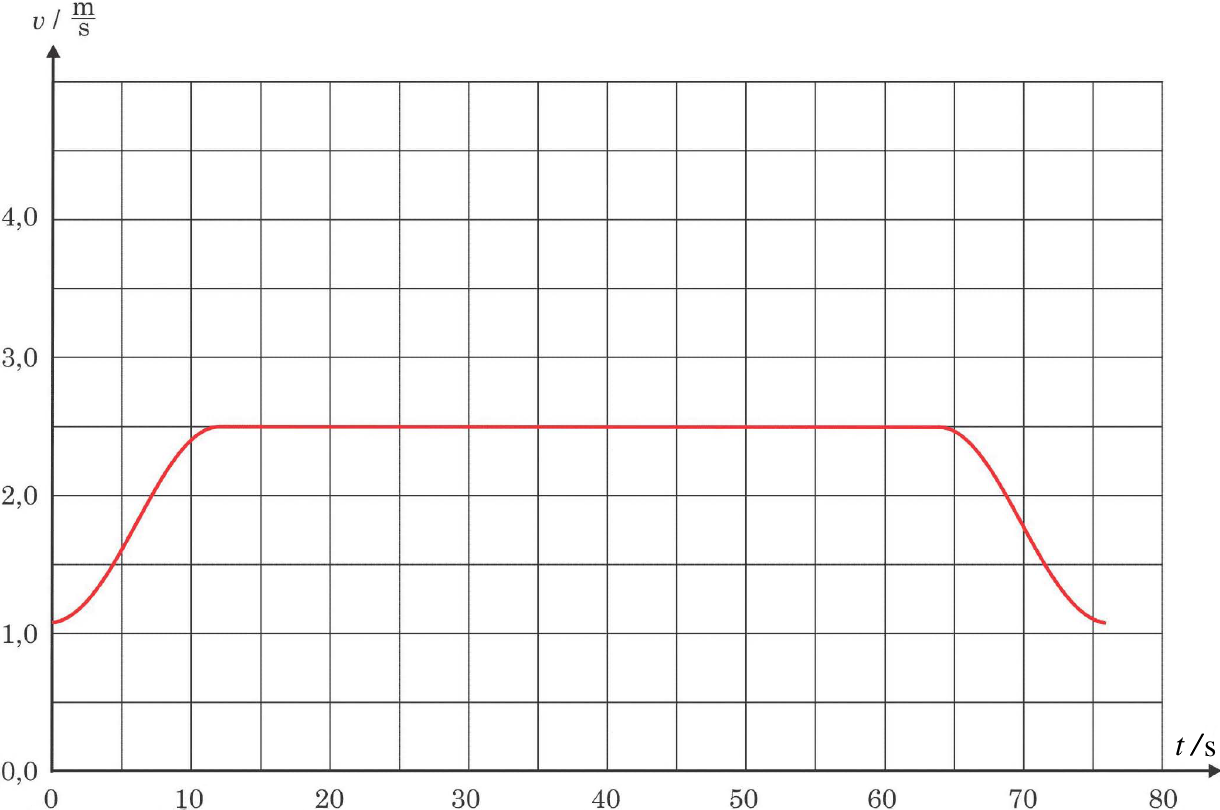
\includegraphics[scale=0.2]{H5_1.png}
\end{center}
\caption{Graf for fodgængerens fart som funktion af tiden.}
\label{fig:1}
\end{figure}
\sol \\ 
\textbf{a.} Vi kan benytte numerisk differentiation med punkterne ved $t=0$ og $t=10$ til at estimere tangentens hældning ved $t=5,0 \;\unit{s} $.
\[
a \approx \frac{(2,4-\frac{4}{3,6})\;\unit{m/s} }{10 \;\unit{s} } \approx 0,13 \;\unit{m/s^2} 
\] 
Altså er accelerationen ved $t=5,0 \;\unit{s} $ cirka $0,13 \;\unit{m/s^2}$. \\[1ex]
\textbf{b.} Længden af det rullende fortov kan bestemmes ved at tælle ternene under grafen. 
Disse tælles til at være cirka 67.
Længden, som hvert tern svarer til er
\[
0,5 \;\unit{m/s} \cdot 5 \;\unit{s}=2,5 \;\unit{m}  
\] 
Længden af fortovet kan nu regnes ud.
\[
s_{\text{fortov}}=67\cdot 2,5 \;\unit{m} \approx 0,17 \;\unit{km} 
\] 
Altså er længden på fortovet $0,17 \;\unit{km} $
\begin{question}{Ind på motorvejen}{}
På en motorvej kører trafikken med $110 \;\unit{km/h} $.
En bil holder stille i nødsporet langs motorvejen.
Bilens fører ønsker at køre ind på motorvejen igen.
Under denne udkørsel accelererer bilen med en konstant acceleration på $1,7 \;\unit{m/s^2} $.
\begin{itemize}
  \item[a.] Hvor lang tid vil det vare, før bilen har opnået farten $110 \;\unit{km/h} $?
\end{itemize}
Føreren af bilen vil undgå, at den bagvedkørende bil skal sagtne farten, når hun kører ind på motorvejen og accelererer op.
\begin{itemize}
  \item[b.] Hvor stort et hul i trafikken skal føreren vente på, når afstanden til den bagvedkørende bil skal være mindst 25 m under hele accelerationen?
\end{itemize}
\end{question}
\sol \\ 
\textbf{a.} Tiden, der går er farten over accelerationen. 
\[
t=\frac{v}{a}=\frac{110 \;\unit{km/h} }{1,7 \;\unit{m/s^2} }\approx 18 \;\unit{s} 
\] 
Altså vil der gå $18 \;\unit{s} $ før bilen har opnået $110 \;\unit{km/h} $.\\[1ex]
\textbf{b.} Vi opstiller en ligning, hvor $h$ er størrelsen på hullet i trafikken, som føreren skal vente på og $s$ er afstanden bilerne mindst skal have under acceleration.
\[
s=h-v\cdot t + \frac{v^2}{2\cdot a}\implies h=s+v\cdot t-\frac{v^2}{2\cdot a}
\] 
Vores værdier kan nu sættes ind i denne.
\[
h=25 \;\unit{m} + 110 \;\unit{km/h} \cdot \frac{110}{3,6\cdot 1,7} \;\unit{s} - \frac{(110 \;\unit{km/h} )^2}{2\cdot 1,7 \;\unit{m/s^2} } \approx 0,29 \;\unit{km} 
\] 
Altså skal hullet i trafikken mindst være $0,29 \;\unit{km} $, hvis afstanden til bagvedkørende bil skal være større end $25 \;\unit{m} $ under accelerationen.

\begin{question}{Skydiving}{}
For at vurdere hvornår faldskærmen skal udløses, foretog en udspringer en måling af farten under et fald fra stor højde. 
  Grafen i \cref{fig:2} viser sammenhængen mellem farten $v$ under den første del af faldet og tiden $t$, der er gået fra udspringets begyndelse.
\begin{itemize}
  \item[a.] Benyt grafen til at bestemme udspringerens acceleration til start, til tiden $5,0 \;\unit{s} $ samt $15 \;\unit{s} $.
  \item[b.] Forklar, hvorfor grafen ser ud som den gør.
\end{itemize}
Faldskærmen udløses, når udspringeren er faldet $2 \;\unit{km} $
\begin{itemize}
  \item[c.] Benyt grafen til at vurdere, hvor lang tid det tager udspringeren at falde $2 \;\unit{km} $
\end{itemize}
\end{question}
\pagebreak
\begin{figure}[h]
\begin{center}
  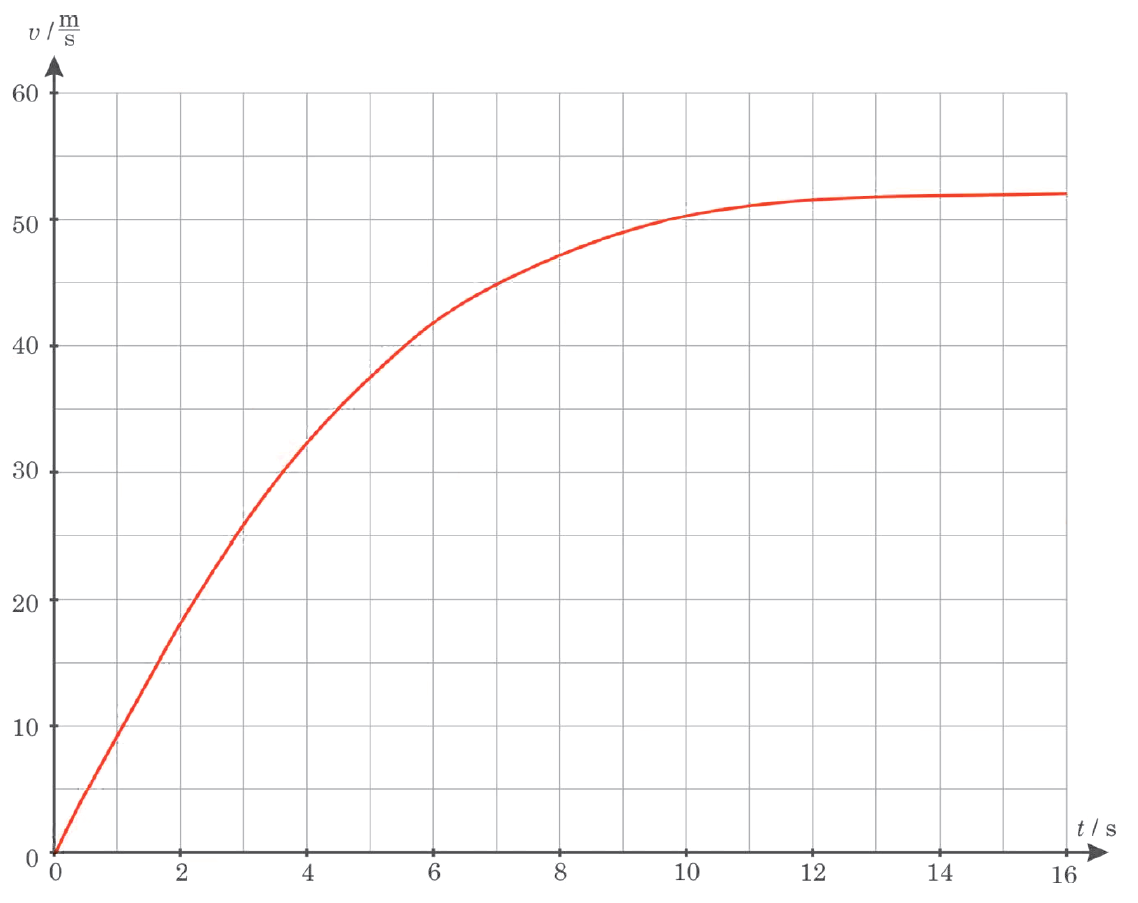
\includegraphics[scale=0.3]{H5_2.png}
\end{center}
\caption{Sammenhængen mellem farten $v$ under den første del af faldet og tiden $t$, der er gået fra udspringets begyndelse.}
\label{fig:2}
\end{figure}
\sol \\ 
\textbf{a.} Den geometriske betydning af accelerationen i dette tilfælde er blot hældningen af tangenten til grafen. 
Disse findes så ved $t=0\;\unit{s}$, $t=5,0 \;\unit{s} $ og $t=10\;\unit{s}$. \\[1ex]
\textbf{b.} Grafen ser ud som den gør, da udspringeren opnår sin terminale fart. På det tidspunkt er opdriften og luftmodstanden lig med kraften, der trækker udspringeren ned mod jorden. \\[1ex]
\textbf{c.} Den geometriske betydning af strækningen, som udspringeren falder, er blot arealet under grafen. Dette estimerer vi ved at tælle tern. Hvert tern er da
\[
1 \;\unit{s} \cdot 5,0 \;\unit{m/s} =5,0 \;\unit{m} 
\] 
Fra $t=0 \;\unit{s} $ til $t=12 \;\unit{s} $ tælles der 88 tern. Vi går ud fra, at $v=52,3 \;\unit{m/s} $, når $t>12 \;\unit{s} $. 
Tiden det tager for udspringeren at falde $2 \;\unit{km} $ må derfor være
\[
t=\frac{2000 \;\unit{m} -88\cdot 5,0 \;\unit{m} }{52,3 \;\unit{m/s} }+12 \;\unit{s} \approx 42 \;\unit{s} 
\] 
Altså tager det udspringeren $42 \;\unit{s} $ at falde $2 \;\unit{km} $.
\end{document}
